\section{射影簇的像}\label{sec:images-of-projective-varieties}

现在到了本章最后一节. 本节的目标是利用先前建立的结果证明以下基本定理.

\begin{Theorem}{射影簇在正则映射下的像是闭的}\leavevmode\label{thm:regular-images-of-projective-varieties-are-closed}
设 $X\subseteq\mathbb{P}^{m}$ 闭, $Y\subseteq\mathbb{P}^{n}$ 为拟射影簇. 若 $F:X\to Y$ 是正则映射, 则 $F(X)$ 在 $Y$ 中闭.
\end{Theorem}

\BookPairedFigure{
这一结果再次说明射影簇是\emph{完备的}, 即它们没有缺失的点: 无论怎样把射影簇映到另一个拟射影簇中, 像总是闭的. Theorem~\ref{thm:regular-images-of-projective-varieties-are-closed} 与仿射情形形成鲜明对比. 如右图所示的仿射双曲线的例子, 投影到仿射直线的映射是正则映射, 其像却不闭. 直观地说, 像中缺少的点反映了双曲线上两支曲线沿其走向无穷远的渐近线.
}{
\phantomsection\label{fig:affine-hyperbola-open-projection}%
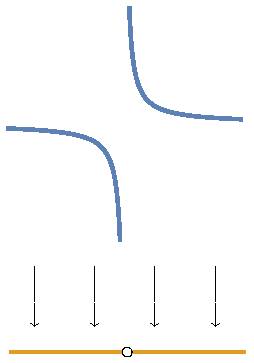
\includegraphics[width=\linewidth]{figures/affine-hyperbola-open-projection.pdf}
}
换一种方式说明仿射簇和射影簇的区别. 回顾在第~\ref{sec:affine-varieties-revisited}~节, 我们特意重新定义\textquotedbl{}仿射簇\textquotedbl{}, 让它不仅指 $\mathbb{A}^{n}$ 的闭子集, 而且指同构于这类子集的拟射影簇. 不过, 可以放心地把\textquotedbl{}射影簇\textquotedbl{}简单定义为 $\mathbb{P}^{n}$ 的一个闭子集, 因为这个概念已经在同构下保持. 的确, 由 Theorem~\ref{thm:regular-images-of-projective-varieties-are-closed} 可推出 (Corollary~\ref{cor:projectivity-invariant-under-quasiprojective-isomorphism}), 若拟射影簇 $X\subseteq\mathbb{P}^{n}$ 同构于另一个射影空间的闭子集, 则 $X$ 在 $\mathbb{P}^{n}$ 中也必是闭的.

本节还将用 Corollary~\ref{cor:regular-functions-on-irreducible-projective-varieties-are-constant} 描述仿射簇和射影簇的另一项区别. 与仿射簇上丰富的多项式函数相比, 不可约射影簇上没有非常值的正则函数. 关键是把 $X$ 上的正则函数看成正则映射 $F:X\to\mathbb{A}^{1}$, 并利用 $\mathbb{A}^{1}$ 的闭子集只有 $\mathbb{A}^{1}$ 本身和有限点集这一事实. $X$ 的不可约性和射影性意味着, 在这些可能性中, $F(X)$ 必是单个点.

有了这些动机, 开始证明 Theorem~\ref{thm:regular-images-of-projective-varieties-are-closed}. 由 Exercise~\ref{ex:image-of-map-is-projection-of-graph}, 从略有不同的角度来看, 正则映射 $F:X\to Y$ 的像 $F(X)$ 满足 $F(X)=\pi(\Gamma_{F})$, 其中 $\Gamma_{F}\subseteq X\times Y$ 是 $F$ 的图像, $\pi$ 是到第二个因子的投影:
\[
  \begin{aligned}
    \pi:X\times Y&\to Y\\
    \pi(x,y)&=y.
  \end{aligned}
\]
由于 $\Gamma_{F}$ 在 $X\times Y$ 中闭 (Proposition~\ref{prop:graphs-of-quasiprojective-regular-maps-are-closed}), 只需证明以下结论.

\begin{Lemma}{从射影簇出发的投影是闭映射}\leavevmode\label{lem:projection-from-projective-factor-is-closed}
若 $X\subseteq\mathbb{P}^{m}$ 闭, $Y\subseteq\mathbb{P}^{n}$ 为拟射影簇, 则投影 $\pi:X\times Y\to Y$ 将 $X\times Y$ 的闭集映为 $Y$ 的闭集.
\end{Lemma}
\begin{Proof}
这个证明颇为复杂, 先作一系列归约. 首先归约到 $X=\mathbb{P}^{m}$ 的情形, 再归约到 $Y$ 为仿射簇的情形, 最后归约到 $Y$ 为 $\mathbb{A}^{n}$ 的情形. 然后在 $X\times Y=\mathbb{P}^{m}\times\mathbb{A}^{n}$ 的情形证明结果.

\textbf{(归约到 $X=\mathbb{P}^{m}$)} 假设引理在 $X=\mathbb{P}^{m}$ 时成立, 令 $X\subseteq\mathbb{P}^{m}$ 闭, 并设 $Z\subseteq X\times Y$ 闭. 由于 $X$ 在 $\mathbb{P}^{m}$ 中闭, $X\times Y$ 在 $\mathbb{P}^{m}\times Y$ 中闭 (Exercise~\ref{ex:product-of-closed-quasiprojective-subvarieties-is-closed}), 因此闭包含
\[
  Z\subseteq X\times Y\subseteq\mathbb{P}^{m}\times Y
\]
表明 $Z$ 在 $\mathbb{P}^{m}\times Y$ 中闭. 若 $\pi:X\times Y\to Y$ 与 $\overline{\pi}:\mathbb{P}^{m}\times Y\to Y$ 分别表示相应的投影, 则由假设 $\overline{\pi}(Z)$ 在 $Y$ 中闭. 但 $\pi(Z)=\overline{\pi}(Z)$, 所以 $\pi(Z)$ 在 $Y$ 中也闭.

这样, $X=\mathbb{P}^{m}$ 的特例蕴含引理的一般情形, 故以下假设 $X=\mathbb{P}^{m}$.

\textbf{(归约到 $Y$ 为仿射簇)} 假设引理在 $Y$ 为仿射簇时成立, 令 $Y$ 为任一拟射影簇. 设 $Z\subseteq\mathbb{P}^{m}\times Y$ 闭. 由于拟射影簇是局部仿射的 (Theorem~\ref{thm:quasiprojective-varieties-have-finite-affine-open-covers}), 对每个 $p\in Y$, 都存在包含 $p$ 的仿射开集 $Y_{p}\subseteq Y$. 将闭集 $Z\subseteq\mathbb{P}^{m}\times Y$ 与 $\mathbb{P}^{m}\times Y_{p}$ 相交, 可见
\[
  Z\cap(\mathbb{P}^{m}\times Y_{p})\subseteq\mathbb{P}^{m}\times Y_{p}
\]
对每个 $p$ 都在 $\mathbb{P}^{m}\times Y_{p}$ 中闭. 因此, 由假设, 在投影 $\pi_{p}:\mathbb{P}^{m}\times Y_{p}\to Y_{p}$ 下的像
\[
  \pi_{p}(Z\cap(\mathbb{P}^{m}\times Y_{p}))\subseteq Y_{p}
\]
在 $Y_{p}$ 中闭. 但 $\pi(Z)\cap Y_{p}=\pi_{p}(Z\cap(\mathbb{P}^{m}\times Y_{p}))$, 所以已证明 $\pi(Z)\cap Y_{p}$ 在 $Y_{p}$ 中闭. 因为这对每个 $p\in Y$ 都成立, 可见 $\pi(Z)$ 在 $Y$ 中局部闭, 因而由 Lemma~\ref{lem:closedness-is-local}, 它在 $Y$ 中闭.

这样, $Y$ 为仿射簇的特例蕴含引理的一般情形, 故以下还假设 $Y$ 为仿射簇.

\textbf{(归约到 $Y=\mathbb{A}^{n}$)} 最后假设引理在 $Y=\mathbb{A}^{n}$ 时成立, 令 $Y\subseteq\mathbb{A}^{n}$ 闭. 设 $Z\subseteq\mathbb{P}^{m}\times Y$ 闭, 注意 $Z$ 作为 $\mathbb{P}^{m}\times\mathbb{A}^{n}$ 的子集也闭. 令 $\pi:\mathbb{P}^{m}\times Y\to Y$ 和 $\overline{\pi}:\mathbb{P}^{m}\times\mathbb{A}^{n}\to\mathbb{A}^{n}$ 分别表示相应的投影. 由于 $\pi(Z)=\overline{\pi}(Z)$, 且由假设 $\overline{\pi}(Z)$ 在 $\mathbb{A}^{n}$ 中闭, 所以 $\pi(Z)$ 在 $Y$ 中闭.

这样, 已将整个引理归约到 $X=\mathbb{P}^{m}$ 和 $Y=\mathbb{A}^{n}$ 的特例. 现在着手证明这一特例. 不过要提醒读者, 下面的论证相当繁复. 在读证明之前或一边读证明一边做下面的 Example~\ref{ex:projecting-closed-set-by-coefficient-matrix}, 可能有助于理解其策略和记号.

\textbf{($X=\mathbb{P}^{m}$ 且 $Y=\mathbb{A}^{n}$ 时的证明)} 设 $Z\subseteq\mathbb{P}^{m}\times\mathbb{A}^{n}$ 闭, 写成
\[
  Z=\mathcal{V}(f_{1},\ldots,f_{\ell}),
\]
其中 $f_{1},\ldots,f_{\ell}\in K[x_{0},\ldots,x_{m},y_{1},\ldots,y_{n}]$. 可以假定每个 $f_{k}$ 关于 $x$ 变量齐次, 并令 $d_{k}$ 表示 $f_{k}$ 关于 $x$ 变量的次数. 注意
\begin{equation}\label{eq:projection-image-nonempty-fibre}
  \pi(Z)=\{b\in\mathbb{A}^{n}\mid\pi^{-1}(b)\cap Z\ne\varnothing\}.
\end{equation}
其余论证的核心是分析条件 $\pi^{-1}(b)\cap Z\ne\varnothing$.

给定 $b=(b_{1},\ldots,b_{n})\in\mathbb{A}^{n}$, 对每个 $k=1,\ldots,\ell$ 定义
\begin{equation}\label{eq:specialize-defining-polynomial-at-affine-point}
  f_{k}^{b}(x_{0},\ldots,x_{m})
  =f_{k}(x_{0},\ldots,x_{m},b_{1},\ldots,b_{n})\in K[x_{0},\ldots,x_{m}].
\end{equation}
自然地将集合
\[
  \pi^{-1}(b)\cap Z
  =\{(a,b)\in\mathbb{P}^{m}\times\{b\}\mid f_{k}^{b}(a)=0\text{ 对所有 }k=1,\ldots,\ell\}
\]
与消没集 $\mathcal{V}(f_{1}^{b},\ldots,f_{\ell}^{b})\subseteq\mathbb{P}^{m}$ 等同. 这样, $\pi^{-1}(b)\cap Z$ 为空的刻画是
\[
  \pi^{-1}(b)\cap Z=\varnothing
  \iff \mathcal{V}(f_{1}^{b},\ldots,f_{\ell}^{b})=\varnothing\subseteq\mathbb{P}^{m}.
\]
由射影零点定理, 条件 $\mathcal{V}(f_{1}^{b},\ldots,f_{\ell}^{b})=\varnothing$ 等价于存在某个 $r\ge0$, 使每个 $r$ 次单项式 $x^{\alpha}$ 都属于 $\langle f_{1}^{b},\ldots,f_{\ell}^{b}\rangle$ (Exercise~\ref{ex:empty-projective-variety-criterion-by-degree}). 为方便起见, 令 $M_{r}$ 为 $x_{0},\ldots,x_{m}$ 的 $r$ 次单项式的指标集, 因而每个 $\alpha\in M_{r}$ 对应一个 $r$ 次单项式 $x^{\alpha}$. 于是, $\pi^{-1}(b)\cap Z=\varnothing$, 当且仅当存在 $r\ge0$, 使对每个 $\alpha\in M_{r}$ 都有
\begin{equation}\label{eq:degree-r-monomial-in-specialized-ideal}
  x^{\alpha}=\sum_{k=1}^{\ell}g_{k}f_{k}^{b},
\end{equation}
其中 $g_{1},\ldots,g_{\ell}\in K[x_{0},\ldots,x_{m}]$. 可用单项式 $x^{\beta}$ 写出 $g_{k}=\sum_{\beta}a_{k,\beta}x^{\beta}$, 从而 \eqref{eq:degree-r-monomial-in-specialized-ideal} 等价于存在 $a_{k,\beta}\in K$ 使
\begin{equation}\label{eq:monomial-expansion-of-specialized-ideal-membership}
  x^{\alpha}=\sum_{k=1}^{\ell}\sum_{\beta}a_{k,\beta}x^{\beta}f_{k}^{b}.
\end{equation}
由于 $\alpha\in M_{r}$ 且 $f_{k}^{b}$ 是 $d_{k}$ 次齐次多项式, 可以假定 \eqref{eq:monomial-expansion-of-specialized-ideal-membership} 的第 $k$ 个加项中出现的每个 $\beta$ 都在 $M_{r-d_{k}}$ 中, 因为所有其他项之和必为零. 对每个 $k\in\{1,\ldots,\ell\}$ 及每个 $\beta\in M_{r-d_{k}}$, 现在把 $x^{\beta}f_{k}^{b}$ 写成单项式的线性组合:
\begin{equation}\label{eq:coefficient-matrix-row-of-specialized-monomial-multiple}
  x^{\beta}f_{k}^{b}=\sum_{\alpha}c_{(k,\beta),\alpha}^{b}x^{\alpha},
\end{equation}
并把这些线性组合的系数排列成矩阵
\[
  C_{r}^{b}=\bigl(c_{(k,\beta),\alpha}^{b}\bigr).
\]
注意 $C_{r}^{b}$ 的列由 $M_{r}$ 编号, 行则由 $(k,\beta)$ 编号, 其中 $\beta\in M_{r-d_{k}}$.

注意, $C_{r}^{b}$ 中由 $(k,\beta)$ 编号的行记录了 $x^{\beta}f_{k}^{b}$ 作为 $\{x^{\alpha}\mid\alpha\in M_{r}\}$ 的线性组合的系数. 因此, 对每个 $\alpha\in M_{r}$ 都存在 \eqref{eq:monomial-expansion-of-specialized-ideal-membership} 中的表示, 等价于标准基向量都在 $C_{r}^{b}$ 的行张成的空间内. 这又等价于 $C_{r}^{b}$ 的秩为 $|M_{r}|$ (即 $C_{r}^{b}$ 的列数). 总结起来, 已证明
\[
  \pi^{-1}(b)\cap Z=\varnothing
  \iff\text{存在 }r\ge0\text{ 使 }\operatorname{rk}(C_{r}^{b})=|M_{r}|.
\]
将以上条件取否定, 得
\[
  \pi^{-1}(b)\cap Z\ne\varnothing
  \iff\text{对每个 }r\ge0,\ \operatorname{rk}(C_{r}^{b})<|M_{r}|.
\]
由此可知, $\pi^{-1}(b)\cap Z\ne\varnothing$ 当且仅当对每个 $r\ge0$, $C_{r}^{b}$ 的所有 $|M_{r}|\times|M_{r}|$ 子式均消没. 这些子式是 $C_{r}^{b}$ 各项的多项式表达式, 而由 \eqref{eq:specialize-defining-polynomial-at-affine-point} 和 \eqref{eq:coefficient-matrix-row-of-specialized-monomial-multiple} 中的定义可知, $C_{r}^{b}$ 的每一项都是 $b_{1},\ldots,b_{n}$ 的多项式表达式. 因此, 所有满足 $\pi^{-1}(b)\cap Z\ne\varnothing$ 的 $b\in\mathbb{A}^{n}$ 构成 $\mathbb{A}^{n}$ 的一个闭子集. 再由 \eqref{eq:projection-image-nonempty-fibre} 得 $\pi(Z)$ 闭, 证明完成.
\end{Proof}

在下一例中, 我们具体说明 Lemma~\ref{lem:projection-from-projective-factor-is-closed} 的证明中用到的一些记号.

\begin{Example}{闭集的投影}\leavevmode\label{ex:projecting-closed-set-by-coefficient-matrix}
为了说明 Lemma~\ref{lem:projection-from-projective-factor-is-closed} 的证明策略, 考察闭子集
\[
  Z=\mathcal{V}(x_{0}+y_{1}x_{1},x_{1}^{2}+y_{2}x_{0}x_{1})
  \subseteq\mathbb{P}^{1}\times\mathbb{A}^{2}
\]
及其在投影 $\pi:\mathbb{P}^{1}\times\mathbb{A}^{2}\to\mathbb{A}^{2}$ 下的像. 首先注意, 例如 $(1,0)\notin\pi(Z)$, 因为在 $Z$ 的定义方程中取 $y_{1}=1$ 和 $y_{2}=0$, 得
\[
  \pi^{-1}(1,0)\cap Z
  =\left\{[a_{0}:a_{1}]\in\mathbb{P}^{1}\ \middle|\
    \substack{a_{0}+a_{1}=0,\\ a_{1}^{2}=0}\right\}=\varnothing.
\]
另一方面, 例如 $(1,1)\in\pi(Z)$, 因为在 $Z$ 的定义方程中取 $y_{1}=y_{2}=1$, 得
\[
  \pi^{-1}(1,1)\cap Z
  =\left\{[a_{0}:a_{1}]\in\mathbb{P}^{1}\ \middle|\
    \substack{a_{0}+a_{1}=0,\\a_{1}^{2}+a_{0}a_{1}=0}\right\}=\{[1:-1]\}.
\]

一般来说, Lemma~\ref{lem:projection-from-projective-factor-is-closed} 的证明表明, $b=(b_{1},b_{2})\in\pi(Z)$ 当且仅当对每个 $r\ge0$, 矩阵 $C_{r}^{b}$ 的所有 $|M_{r}|\times|M_{r}|$ 子式都为零. 为了理解这一叙述, 特别是理解这些记号, 我们显式计算 $r=3$ 时的矩阵.

为对一般的 $b=(b_{1},b_{2})$ 计算矩阵 $C_{3}^{b}$, 首先考察多项式
\[
  f_{1}^{b}=x_{0}+b_{1}x_{1}\qquad\text{和}\qquad f_{2}^{b}=x_{1}^{2}+b_{2}x_{0}x_{1}.
\]
将这两个多项式各自乘以所有能使乘积关于 $x$ 变量为三次的 $x_{0},x_{1}$ 的单项式, 并记录结果中单项式 $x_{0}^{3}$, $x_{0}^{2}x_{1}$, $x_{0}x_{1}^{2}$ 和 $x_{1}^{3}$ 的系数, 得到
\[
  \begin{aligned}
  f_{1}^{b}\cdot x_{0}^{2}&=\boxed{1}\cdot x_{0}^{3}+\boxed{b_{1}}\cdot x_{0}^{2}x_{1}
        +\boxed{0}\cdot x_{0}x_{1}^{2}+\boxed{0}\cdot x_{1}^{3}\\
  f_{1}^{b}\cdot x_{0}x_{1}&=\boxed{0}\cdot x_{0}^{3}+\boxed{1}\cdot x_{0}^{2}x_{1}
        +\boxed{b_{1}}\cdot x_{0}x_{1}^{2}+\boxed{0}\cdot x_{1}^{3}\\
  f_{1}^{b}\cdot x_{1}^{2}&=\boxed{0}\cdot x_{0}^{3}+\boxed{0}\cdot x_{0}^{2}x_{1}
        +\boxed{1}\cdot x_{0}x_{1}^{2}+\boxed{b_{1}}\cdot x_{1}^{3}\\
  f_{2}^{b}\cdot x_{0}&=\boxed{0}\cdot x_{0}^{3}+\boxed{b_{2}}\cdot x_{0}^{2}x_{1}
        +\boxed{1}\cdot x_{0}x_{1}^{2}+\boxed{0}\cdot x_{1}^{3}\\
  f_{2}^{b}\cdot x_{1}&=\boxed{0}\cdot x_{0}^{3}+\boxed{0}\cdot x_{0}^{2}x_{1}
        +\boxed{b_{2}}\cdot x_{0}x_{1}^{2}+\boxed{1}\cdot x_{1}^{3}.
  \end{aligned}
\]
则 $C_{3}^{b}$ 是由方框中的各项构成的 $5\times4$ 矩阵, 这矩阵的 $4\times4$ 子式消没是 $b$ 属于 $\pi(Z)$ 的必要条件. 其中一个子式是删去 $C_{3}^{b}$ 的第四行所得矩阵的行列式, 读者可以核对它等于
\[
  1-b_{1}b_{2}.
\]
特别地, 元素 $b=(b_{1},b_{2})\in\pi(Z)$ 必须满足 $b_{1}b_{2}=1$, 这和我们算出的 $(1,0)\notin\pi(Z)$ 但 $(1,1)\in\pi(Z)$ 一致.

由 $C_{3}^{b}$ 的其他子式以及其他 $r\ge1$ 的 $C_{r}^{b}$ 的子式消没, 还得到关于 $b_{1},b_{2}$ 的更多条件. 不过, 实际上它们都由单一条件 $b_{1}b_{2}=1$ 蕴含. 可直接由 $\pi(Z)$ 的定义核验这一点: 它由所有满足
\[
  a_{0}+b_{1}a_{1}=0=a_{1}^{2}+b_{2}a_{0}a_{1}
  \qquad\text{对某个 }[a_{0}:a_{1}]\in\mathbb{P}^{1}
\]
的点 $(b_{1},b_{2})\in\mathbb{A}^{2}$ 组成. 这个方程组很容易解得 $b_{1}b_{2}=1$. 因此, 无论用这一直接计算, 还是用上面说明的子式方法, 都得到 $\pi(Z)$ 确实是一个闭集: $\pi(Z)=\mathcal{V}(y_{1}y_{2}-1)\subseteq\mathbb{A}^{2}$.
\end{Example}

Theorem~\ref{thm:regular-images-of-projective-varieties-are-closed} 的证明现在可由 Lemma~\ref{lem:projection-from-projective-factor-is-closed} 很快得到.
\begingroup
\renewcommand{\AJProofBegin}{%
  \par\addvspace{\topsep}\noindent
  {\sffamily\bfseries\CJKfamily{pffont}Proof of Theorem~\ref{thm:regular-images-of-projective-varieties-are-closed}}\enspace\ignorespaces
}
\begin{Proof}
由于 $F(X)=\pi(\Gamma_{F})$, 且由 Proposition~\ref{prop:graphs-of-quasiprojective-regular-maps-are-closed} 知 $\Gamma_{F}\subseteq X\times Y$ 在 $X\times Y$ 中闭, 由 Lemma~\ref{lem:projection-from-projective-factor-is-closed} 可知 $F(X)$ 在 $Y$ 中闭.
\end{Proof}
\endgroup

现在验证本节开头提到的 Theorem~\ref{thm:regular-images-of-projective-varieties-are-closed} 的两个重要推论.

\begin{Corollary}{在射影空间中闭是内在性质}\leavevmode\label{cor:projectivity-invariant-under-quasiprojective-isomorphism}
若 $X\subseteq\mathbb{P}^{m}$ 和 $Y\subseteq\mathbb{P}^{n}$ 是同构的拟射影簇, 则 $X$ 在 $\mathbb{P}^{m}$ 中闭, 当且仅当 $Y$ 在 $\mathbb{P}^{n}$ 中闭.
\end{Corollary}
\begin{Proof}
设 $X$ 在 $\mathbb{P}^{m}$ 中闭, 且 $F:X\to Y$ 为同构. 可以把 $F$ 视为从 $X$ 到 $\mathbb{P}^{n}$ 的正则映射, 由 Theorem~\ref{thm:regular-images-of-projective-varieties-are-closed} 可知 $F(X)$ 在 $\mathbb{P}^{n}$ 中闭. 但因 $F$ 是同构, $F(X)=Y$, 所以 $Y$ 在 $\mathbb{P}^{n}$ 中闭. 双向陈述由对称性得到.
\end{Proof}

\begin{Corollary}{射影簇上的正则函数}\leavevmode\label{cor:regular-functions-on-irreducible-projective-varieties-are-constant}
若 $X$ 为不可约射影簇, 则 $X$ 上每个正则函数都为常值. 换句话说, $K[X]=K$.
\end{Corollary}
\begin{Proof}
正则函数 $F:X\to K$ 与正则映射 $F:X\to\mathbb{A}^{1}$ 相同, 所以 Theorem~\ref{thm:regular-images-of-projective-varieties-are-closed} 蕴含 $F(X)\subseteq\mathbb{A}^{1}$ 是闭的. $\mathbb{A}^{1}$ 的非空闭子集只有整个 $\mathbb{A}^{1}$ 和有限点集. 不可能有 $F(X)=\mathbb{A}^{1}$, 因为如果如此, 将 $F$ 与包含映射 $j_{0}:\mathbb{A}^{1}\to\mathbb{P}^{1}$ 复合会给出正则映射 $X\to\mathbb{P}^{1}$, 其像等于 $\mathbb{A}^{1}\subseteq\mathbb{P}^{1}$, 而这个像并不闭.

因此, $F$ 的像必为有限点集 $a_{1},\ldots,a_{\ell}\in\mathbb{A}^{1}$, 意味着
\[
  X=F^{-1}(a_{1})\sqcup\cdots\sqcup F^{-1}(a_{\ell}).
\]
这个不交并中的每个集合都在 $X$ 中闭 (Theorem~\ref{thm:regular-maps-are-zariski-continuous}), 所以 $X$ 的不可约性蕴含必有 $\ell=1$. 换句话说, $F(X)$ 只由一个元素组成, 所以 $F$ 是常值函数.
\end{Proof}

本节最后回到一个熟悉的例子.

\begin{Example}{$\mathbb{A}^{2}\setminus\{(0,0)\}$ 不是射影簇}\leavevmode\label{ex:punctured-affine-plane-is-not-projective}
如在 Example~\ref{ex:punctured-affine-plane-is-not-affine} 中看到的, 拟射影簇 $\mathbb{A}^{2}\setminus\{(0,0)\}$ 不同构于仿射簇. 现在也可以验证它不同构于射影簇. 我们给出两种论证, 分别依赖刚证明的关于射影簇的两个推论之一.

第一种论证基于 $\mathbb{A}^{2}\setminus\{(0,0)\}\subseteq\mathbb{P}^{2}$ 不闭这一事实. 的确, $\mathbb{A}^{2}\setminus\{(0,0)\}$ 是 $\mathbb{P}^{2}$ 的非空开子集, 从而稠密. 因此它只有在等于整个 $\mathbb{P}^{2}$ 时才可能闭, 但它并不等于整个 $\mathbb{P}^{2}$. 由于 $\mathbb{A}^{2}\setminus\{(0,0)\}$ 在 $\mathbb{P}^{2}$ 中不闭, Corollary~\ref{cor:projectivity-invariant-under-quasiprojective-isomorphism} 蕴含它不同构于射影簇.

第二种论证基于 Example~\ref{ex:punctured-affine-plane-is-not-affine} 中的观察:
\[
  K[\mathbb{A}^{2}\setminus\{(0,0)\}]=K[x,y].
\]
由于 $\mathbb{A}^{2}\setminus\{(0,0)\}$ 的正则函数环并不只是常值函数 $K$, 由 Corollary~\ref{cor:regular-functions-on-irreducible-projective-varieties-are-constant} 可知 $\mathbb{A}^{2}\setminus\{(0,0)\}$ 不可能同构于射影簇.
\end{Example}

本章开始熟悉拟射影簇的理论. 重要的是, 现在已经精确说明仿射簇和射影簇如何处在这一更一般的框架之中. 在下一章, 即本书最后一章, 我们转向拟射影簇的若干关键性质, 如维数和光滑性. 在本章工作的基础上, 我们会看到, 利用拟射影簇的局部仿射性质, 不需太多额外工作, 就能直接从仿射情形引入这些性质的基本特征.

\BookExerciseHeading
\begin{BookExercises}
  \item\label{ex:image-of-map-is-projection-of-graph} 令 $F:X\to Y$ 为集合之间的函数, $\Gamma_{F}\subseteq X\times Y$ 为 $F$ 的图像. 证明 $F(X)=\pi(\Gamma_{F})$, 其中 $\pi:X\times Y\to Y$ 为投影映射.
  \item\label{ex:coefficient-matrix-for-quadratic-multiples-in-projection-example} 令 $Z\subseteq\mathbb{P}^{1}\times\mathbb{A}^{2}$ 如 Example~\ref{ex:projecting-closed-set-by-coefficient-matrix} 所示, 计算矩阵 $C_{2}^{b}$. 这个矩阵的子式消没给出 $b\in\pi(Z)$ 的哪些条件? 验证当 $b_{1}b_{2}=1$ 时这些条件都满足, 如 Example~\ref{ex:projecting-closed-set-by-coefficient-matrix} 所断言.
  \item\label{ex:projection-of-common-root-of-two-linear-forms} 令 $Z=\mathcal{V}(x_{0}+y_{1}x_{1},x_{0}+y_{2}x_{1})\subseteq\mathbb{P}^{1}\times\mathbb{A}^{2}$, 令 $\pi:\mathbb{P}^{1}\times\mathbb{A}^{2}\to\mathbb{A}^{2}$ 表示投影.
  \begin{enumerate}
    \item 直接计算像 $\pi(Z)$.
    \item 计算矩阵 $C_{1}^{b}$ 和 $C_{2}^{b}$, 并确认当 $b\in\pi(Z)$ 时, 它们的所有最大阶子式均消没.
  \end{enumerate}
  \item\label{ex:regular-map-from-projective-to-affine-is-constant} 证明从不可约射影簇到仿射簇的每个正则映射都是常值的.
  \item\label{ex:projective-line-times-affine-line-is-neither-affine-nor-projective} 证明 $\mathbb{P}^{1}\times\mathbb{A}^{1}$ 既不 (同构于) 仿射簇, 也不 (同构于) 射影簇.
  \item\label{ex:punctured-projective-plane-is-neither-affine-nor-projective} 证明 $\mathbb{P}^{2}\setminus\{[1:0:0]\}$ 既不 (同构于) 仿射簇, 也不 (同构于) 射影簇.
  \item\label{ex:projective-line-endomorphism-constant-or-surjective} 证明每个正则映射 $\mathbb{P}^{1}\to\mathbb{P}^{1}$ 或为常值, 或为满射.
\end{BookExercises}
